%%%%%%%%%%%%%%%%%%%%%%%%%%%%%%%%%%%%%%%%%%%%%%%%%%%%%%%%%%%%%%%%%%%%%%
\begin{frame}[fragile]\frametitle{}
\begin{center}
{\Large Computational Complexity}
\end{center}

\end{frame}

\begin{frame}
	\frametitle{Time complexity}
	\framesubtitle{XKCD Algorithms: \url{https://xkcd.com/1667}}
	
	\begin{center}
		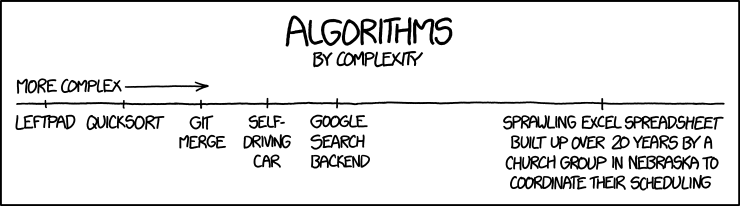
\includegraphics[width=0.9\textwidth]{images/algorithms.png}
	\end{center}
\end{frame}


\begin{frame}
	\frametitle<-3>{What does it do?}
	\frametitle<4->{How fast does it do it?}

	\begin{overlayarea}{\textwidth}{\textheight}
		\lstinputlisting{src/for-loop.py}
		\pause
		\only<2-3>{
			\begin{block}{What does it do?}
				What does the code compute?
			\end{block}
			\only<3->{
				\begin{block}{Sum of squares}
					\texttt{foo(n)} computes $\sum\limits_{i=0}^{n-1} i^2$
				\end{block}
			}
		}
		\only<4->{
			\begin{block}{How fast does it do it?}
				How fast is it?
			\end{block}
			\only<5->{
				\begin{alertblock}{Harder to answer}
					1 second for $n=1000$.\\
					\only<6->{
						But what if $n$ changes?\\
						And what if we use another computer?
					}
				\end{alertblock}	
			}
		}
	\end{overlayarea}
\end{frame}

\begin{frame}
	\frametitle{Why do we ask this?}

	\begin{columns}
		\column{0.455\textwidth}
			\lstinputlisting{src/for-loop.py}
			\lstinputlisting{src/nested-for-loop.py}
		\column{0.455\textwidth}
		\pause
		\begin{block}{Comparing implementations}
			How can we compare \texttt{foo} and \texttt{bar}?
		\end{block}
		\pause
		\begin{block}{Counting}
			By counting operations!
		\end{block}
	\end{columns}
\end{frame}

\begin{frame}
	\frametitle{Counting operations}
	\begin{columns}
		\column{0.455\textwidth}
			\lstinputlisting{src/for-loop.py}
		\column{0.455\textwidth}
		\pause
		\begin{block}{Counting operations}
			How many operations happen when we call \texttt{foo(n)}?
			\begin{enumerate}[A.]
				\item $2 + n$
				\item $2 + n + n$
				\item $3 + 2n + n-1$
				\item $4 + n + n + n + n-1$
			\end{enumerate}
		\end{block}
	\end{columns}
	\pause
	\begin{block}{Counting}
		It depends\dots
	\end{block}
\end{frame}

\begin{frame}
	\frametitle{Getting rid of those nasty constants}

	\begin{itemize}
		\item Observation: We do not care if it's is $2+n$ or even $3+2n$.
		\item The important part is that it \textit{scales with the input}.
			\pause
		\item We call this the ``asymptotic run time complexity''.
	\end{itemize}
	\pause
	\lstinputlisting{src/for-loop.py}

	\begin{block}{No more numbers}
		We say this code has $c_0 + c_1n$ operations, where:
		\begin{itemize}
			\item $c_0$ is initialisation of $s$ on line 2 and the return statement on line 5.
			\item $c_1$ is the \texttt{range} function on line 3 and the multiplication and addition on line 4.
		\end{itemize}
	\end{block}
\end{frame}

\begin{frame}
	\frametitle{Getting rid of those nasty constants}

	\begin{overlayarea}{\textwidth}{\textheight}
			\lstinputlisting{src/nested-for-loop.py}
			\only<1>{
			\begin{block}{So what about here?}
				How can we describe the number of operations here?	
			\end{block}
		}
		\only<2>{
			\begin{block}{Quadratic time}
				We say this code has $c_0 + c_1n + c_2 n^2$ operations, where:
				\begin{itemize}
					\item $c_0$ is initialisation of $s$ on line 2 and the return statement on line 6.
					\item $c_1$ is the \texttt{range} function on line 3.
					\item $c_2$ is the \texttt{range} function on line 4 and the multiplication and addition on line 5.
				\end{itemize}
			\end{block}
		}
	\end{overlayarea}
\end{frame}

\begin{frame}
	\frametitle{So why does this matter?}
	\framesubtitle{Observing the differences}
\end{frame}

\begin{frame}
	\frametitle{Some numbers!}
	\framesubtitle{Check the code used to find these numbers on GitLab!}
	
	\begin{exampleblock}{Differences in run time}

		Different code snippets, all executed 1000 times.

		\hfill\\
		\begin{tabular}{c | c c c c c c c}
			\small
			Input size & constant & linear & quadratic & cubic & exponential & factorial\\
			\midrule
			\pause
			1 & $<$10 ms & $<$10 ms & $<$10 ms & $<$10 ms & $<$10 ms & $<$10 ms\\
			2 & $<$10 ms & $<$10 ms & $<$10 ms & $<$10 ms & $<$10 ms & $<$10 ms\\
			\pause
			5 & $<$10 ms & $<$10 ms & $<$10 ms & 36 ms & 40 ms & 210 ms\\
			\pause
			7 & $<$10 ms & $<$10 ms & $<$10 ms & 49 ms & 50 ms & \alert{$>$3000 ms} \\
			\pause
			10 & $<$10 ms & $<$10 ms & 23 ms & 78 ms & 84 ms & \alert{$>$3000 ms}\\
			\pause
			100 & $<$10 ms & $<$10 ms & 284 ms & \alert{$>$3000 ms} & \alert{$>$3000 ms} & \alert{$>$3000 ms} \\
			\pause
			1000 & $<$10 ms & 54 ms & \alert{$>$3000 ms} &\alert{$>$3000 ms} & \alert{$>$3000 ms} & \alert{$>$3000 ms} \\
			\pause
			10000 & $<$10 ms &  \alert{$>$3000 ms} &\alert{$>$3000 ms} &\alert{$>$3000 ms} & \alert{$>$3000 ms} & \alert{$>$3000 ms} \\
		\end{tabular}
	\end{exampleblock}	
\end{frame}

\begin{frame}
	\frametitle{Classifying these run times}
	\framesubtitle{XKCD: Formal Logic \url{https://xkcd.com/1033}}

	\begin{center}
	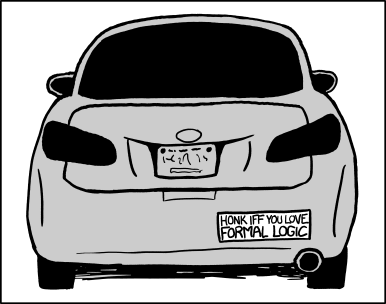
\includegraphics[width=0.6\textwidth]{images/formal_logic.png}
	\end{center}
\end{frame}

\begin{frame}
	\frametitle{Big-Oh notation}

	\begin{itemize}
		\item We care about what we call: ``asymptotic run time complexity''.
		\item We denote this using big-Oh, e.g.\ $f(n) = 3n + 2$ is $O(n)$.
	\end{itemize}
	\pause
	\begin{block}{A friend of mine told me...}
		Have you seen this notation before?
	\end{block}
	\pause
	\begin{block}{Something something, mathematics?}
	\begin{itemize}
		\item You (may?) have used big-Oh to a certain point before. E.g.\ as $n$ approaches $5$.
			\pause
		\item In computer science we only think about when $n$ approaches $\infty$.
	\end{itemize}
	\end{block}
\end{frame}

\begin{frame}
	\frametitle{Formally}
	\begin{definition}[Big-Oh]
		A function $f(n)$ is $O(g(n))$ iff there is a positive real constant $c$ and a positive integer $n_0$ such that for
		all $n \geq n_0$ it holds that $f(n) \leq c g(n)$. In other words:\\
		$\exists c \in \mathbb{R}, \exists n_0 \in \mathbb{N} (c > 0 \wedge n_0 \geq 1 \wedge (\forall n \in \mathbb{N} (n
		\geq n_0 \to f(n) \leq cg(n))))$.
	\end{definition}
	\pause
	\begin{block}{So...}
		Which of the following is/are true?
		\begin{enumerate}[A.]
			\item $n^2$ is $O(n^3)$
			\item $8n^2$ is $O(n^2)$
			\item $16n^2 + 5n + 2$ is $O(n^2)$
			\item $16n^2 + 5n \log n$ is $O(n^2)$
			\item $16n^2\log n$ is $O(n^2)$
		\end{enumerate}
	\end{block}
\end{frame}

\begin{frame}
	\frametitle{Let's prove that shall we?}
	\framesubtitle{Well, I say ``we''...}

	\begin{block}{}
		Prove that $f(n) = 16n^2 + 5n + 2$ is $O(n^2)$.
	\end{block}
	\pause
	\begin{proof}
		To prove: $\exists c > 0, n_0 \geq 1$ such that $\forall n \geq n_0$ $16n^2 + 5n + 2 \leq cn^2$.\\
		\pause
		Take $n_0 = 1$, now for all $n \in \mathbb{N}$ with $n \geq n_0$:
		\begin{align*}
			16n^2 + 5n + 2 &\leq 16n^2 + 5n^2 + 2n^2 \\
										 &= 23n^2
		\end{align*}
		So take $c=23$.
	\end{proof}
\end{frame}

\begin{frame}
	\frametitle{Polynomial run time}
	
	\begin{definition}[Polynomial run time]
		A function has a polynomial run time $T(n)$ if $T(n)$ is $O(n^c)$ for some constant $c$.	
	\end{definition}
	\pause
	\begin{exampleblock}{This course}
		Most of the algorithms treated in this course have a polynomial run time.
	\end{exampleblock}	

	\pause
	\begin{alertblock}{Remember this}
		We will revisit the notion of polynomial run times in the very last lecture, where we study some problems that
		we believe to have no polynomial time solution!
	\end{alertblock}	
\end{frame}

\begin{frame}
	\frametitle{Some numbers! Revisited}
	\framesubtitle{Check the code used to find these numbers on GitLab!}
	
	\begin{exampleblock}{Differences in run time}

		We can now formalise our previous table a little bit:
		\pause

		\hfill\\
		\begin{tabular}{c | c c c c c c c}
			\small
			Input size & \alert{$O(1)$} & \alert{$O(n)$} & \alert{$O(n^2)$} & \alert{$O(n^3)$} & \alert{$O(2^n)$} & \alert{$O(n!)$} \\
			\midrule
			1 & $<$10 ms & $<$10 ms & $<$10 ms & $<$10 ms & $<$10 ms & $<$10 ms\\
			2 & $<$10 ms & $<$10 ms & $<$10 ms & $<$10 ms & $<$10 ms & $<$10 ms\\
			5 & $<$10 ms & $<$10 ms & $<$10 ms & 36 ms & 40 ms & 210 ms\\
			7 & $<$10 ms & $<$10 ms & $<$10 ms & 49 ms & 50 ms & $>$3000 ms \\
			10 & $<$10 ms & $<$10 ms & 23 ms & 78 ms & 84 ms & $>$3000 ms\\
			100 & $<$10 ms & $<$10 ms & 284 ms & $>$3000 ms & $>$3000 ms & $>$3000 ms \\
			1000 & $<$10 ms & 54 ms & $>$3000 ms &$>$3000 ms & $>$3000 ms & $>$3000 ms \\
			10000 & $<$10 ms &  $>$3000 ms &$>$3000 ms &$>$3000 ms & $>$3000 ms & $>$3000 ms \\
		\end{tabular}
		\pause
		\hfill\\
		Next lecture we will finish formalising this table.
	\end{exampleblock}	
\end{frame}

\begin{frame}
	\frametitle{Revisiting our code snippets}
	
	\lstinputlisting{src/for-loop.py}
	\begin{columns}
		\column{0.455\textwidth}
	\begin{block}{So which is it?}
		Which of these describes the run time $T(n)$?
	\begin{enumerate}[A.]
		\item $T(n)$ is $O(1)$.
		\item $T(n)$ is $O(n)$. 
		\item $T(n)$ is $O(n^2)$. 
		\item $T(n)$ is $O(n^3)$. 
		\item I don't know.
	\end{enumerate}	
	\end{block}
		\column{0.455\textwidth}
		\pause
		\begin{block}{Multiple correct answers}
			B through D are correct.
		\end{block}
		\pause
			\begin{block}{Tightest bound}
				We often request the tightest bound. Which in this case is $O(n)$.
			\end{block}	
	\end{columns}
\end{frame}

\begin{frame}
	\frametitle{Which case?}
	\lstinputlisting{src/for-loop-wc.py}
	\begin{columns}
		\column{0.755\textwidth}
	\begin{block}{So which is it?}
		Which of these forms a tight bound on the run time $T(n)$?
	\begin{enumerate}[A.]
		\small
		\item $O(1)$. 
		\item $O(n)$. 
		\item $O(n^2)$. 
		\item I don't know.
	\end{enumerate}	
	\end{block}
		\column{0.255\textwidth}
		\pause
		\begin{block}{}
			Only B
		\end{block}
		\pause
			\begin{block}{Worst Kaas}
				We talk about the \textit{worst-case}.
			\end{block}	
	\end{columns}
\end{frame}

% \begin{frame}
	% \frametitle{So...}
	% \framesubtitle{There and back again}

	% \begin{columns}
		% \column{0.455\textwidth}
			% \lstinputlisting{src/for-loop.py}
			% \lstinputlisting{src/nested-for-loop.py}
		% \column{0.455\textwidth}
		% \begin{block}{Comparing implementations}
			% How can we compare \texttt{foo} and \texttt{bar}?
		% \end{block}
		% \begin{block}{Counting}
			% \st{By counting operations!}\\
			% \pause
			% By comparing their asymptotic run time complexity!
		% \end{block}
		% \begin{block}{Issues?}
			% What are the limitations?
		% \end{block}
	% \end{columns}
% \end{frame}

\begin{frame}
	\frametitle{Space complexity}
	\framesubtitle{Anywhere in space and time}
	\begin{center}
		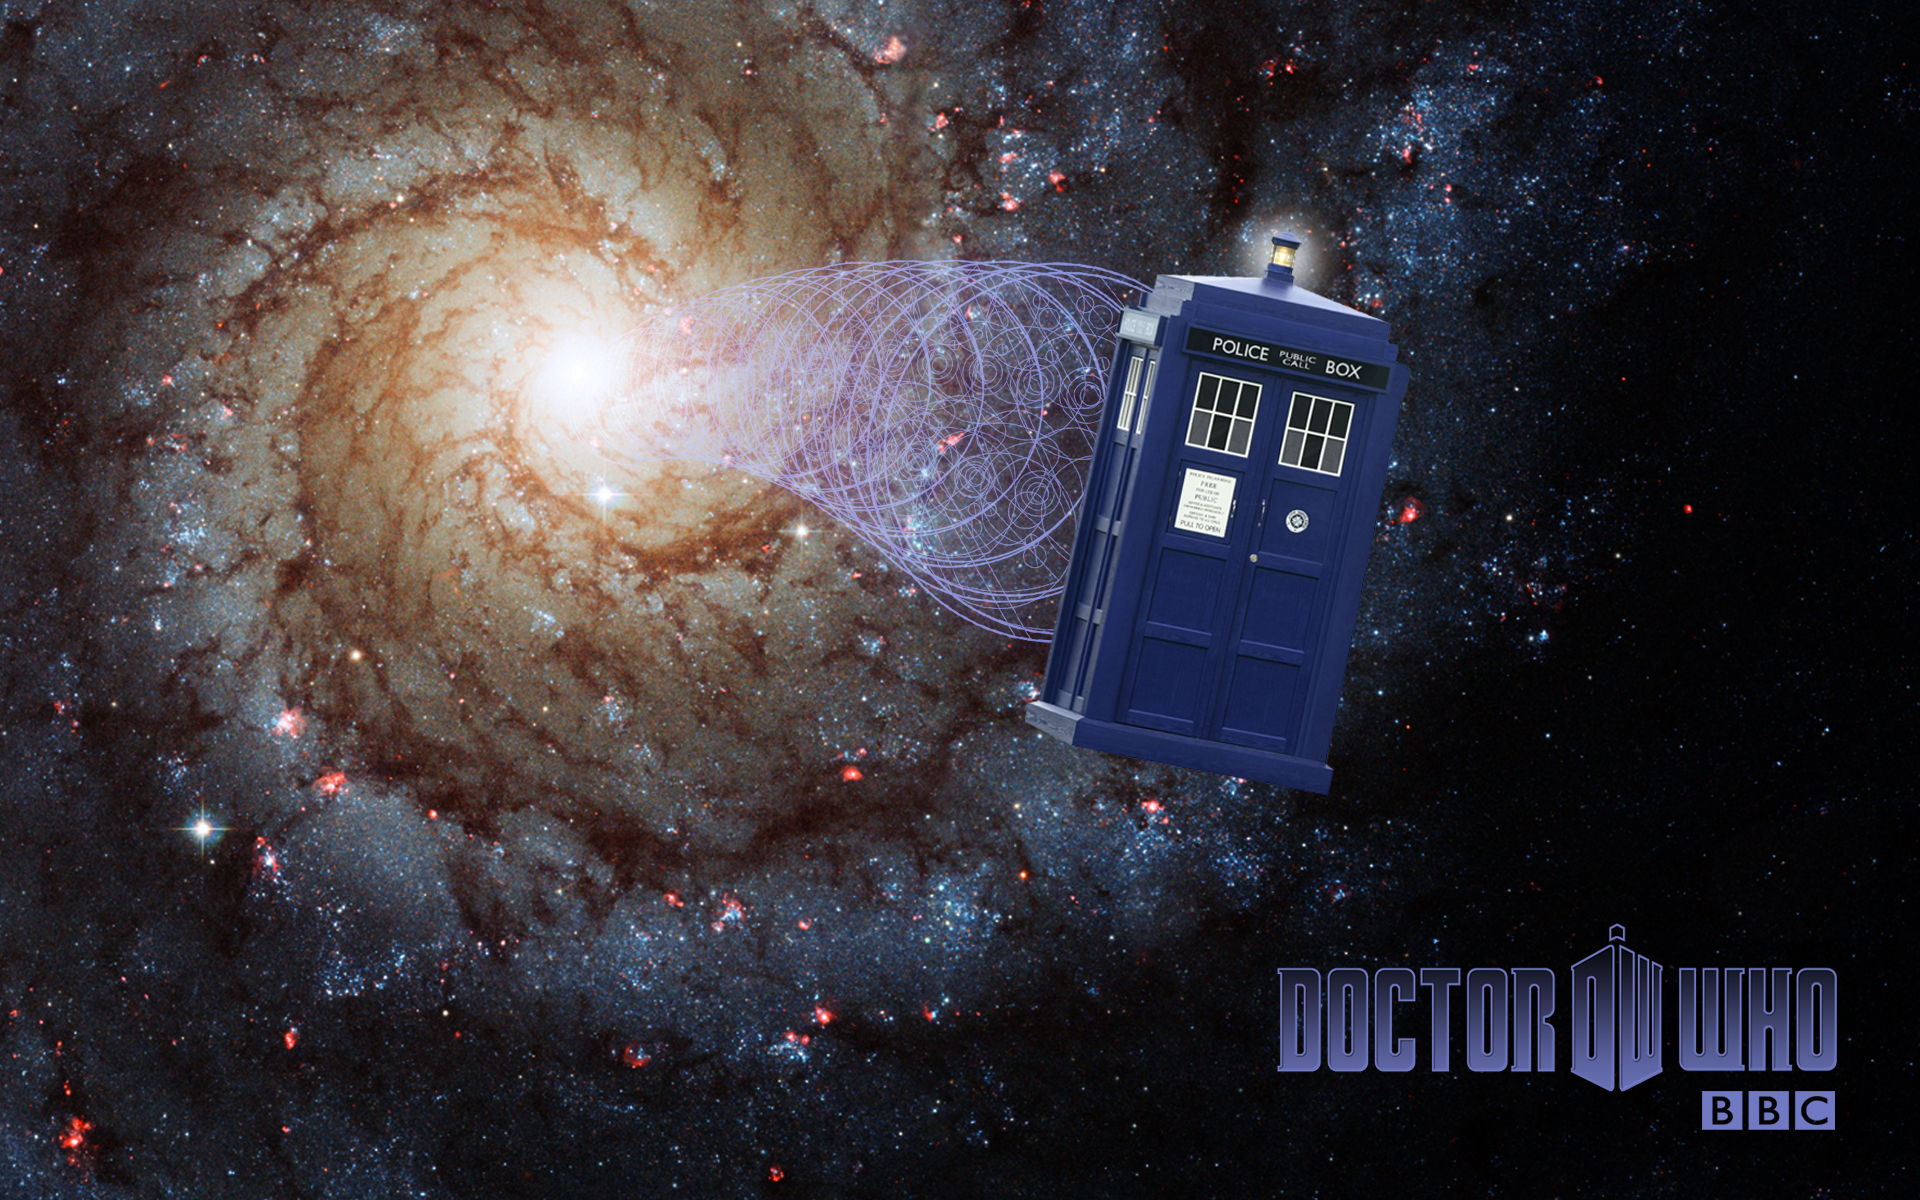
\includegraphics[width=0.73\textwidth]{images/tardis.jpg}\\
		\hspace*{15pt}\hbox{\scriptsize Image By:\thinspace{\itshape anna\_thetical}}
		%https://www.flickr.com/photos/anna_thetical/4147623095
	\end{center}
\end{frame}

\begin{frame}
	\frametitle{Space complexity}
	\begin{itemize}
		\item So far we have only looked at the required \alert{time} of a function.
		\item What about the required \alert{space}?
			\pause
		\item Just like time, space is a \alert{finite} resource.	
		\item So it is important to be able to set bounds on the usage.
	\end{itemize}
	\pause
	\begin{block}{Difference?}
		Is there any difference in how time and space are used by functions?
	\end{block}
	\pause
	\begin{block}{Recycling}
		Yes! Space can be reused, whereas time cannot.
	\end{block}
\end{frame}

\begin{frame}
	\frametitle{A first example}
	\framesubtitle{Creating a list}
	
	\begin{columns}
		\column{0.455\textwidth}
			\lstinputlisting{src/comprehension-complexity.py}
		\column{0.455\textwidth}
		\pause
		\begin{block}{Space}
			What is the \alert{space} complexity of this list comprehension?
			\begin{enumerate}[A.]
				\item $\Theta(1)$
				\item $\Theta(n)$ 
				\item $\Theta(n^2)$
				\item I don't know.
			\end{enumerate}
		\end{block}
	\end{columns}
	\pause
	\begin{block}{Linear time}
		We have $n$ integers, each requiring some constant amount of space $c$. Thus $S(n) = cn$, so $\Theta(n)$ space is
		required.
	\end{block}
\end{frame}

\begin{frame}
	\frametitle{Memory in a computer}
	\framesubtitle{The following slides are based on slides originally created by Robbert Krebbers}
\begin{center}
	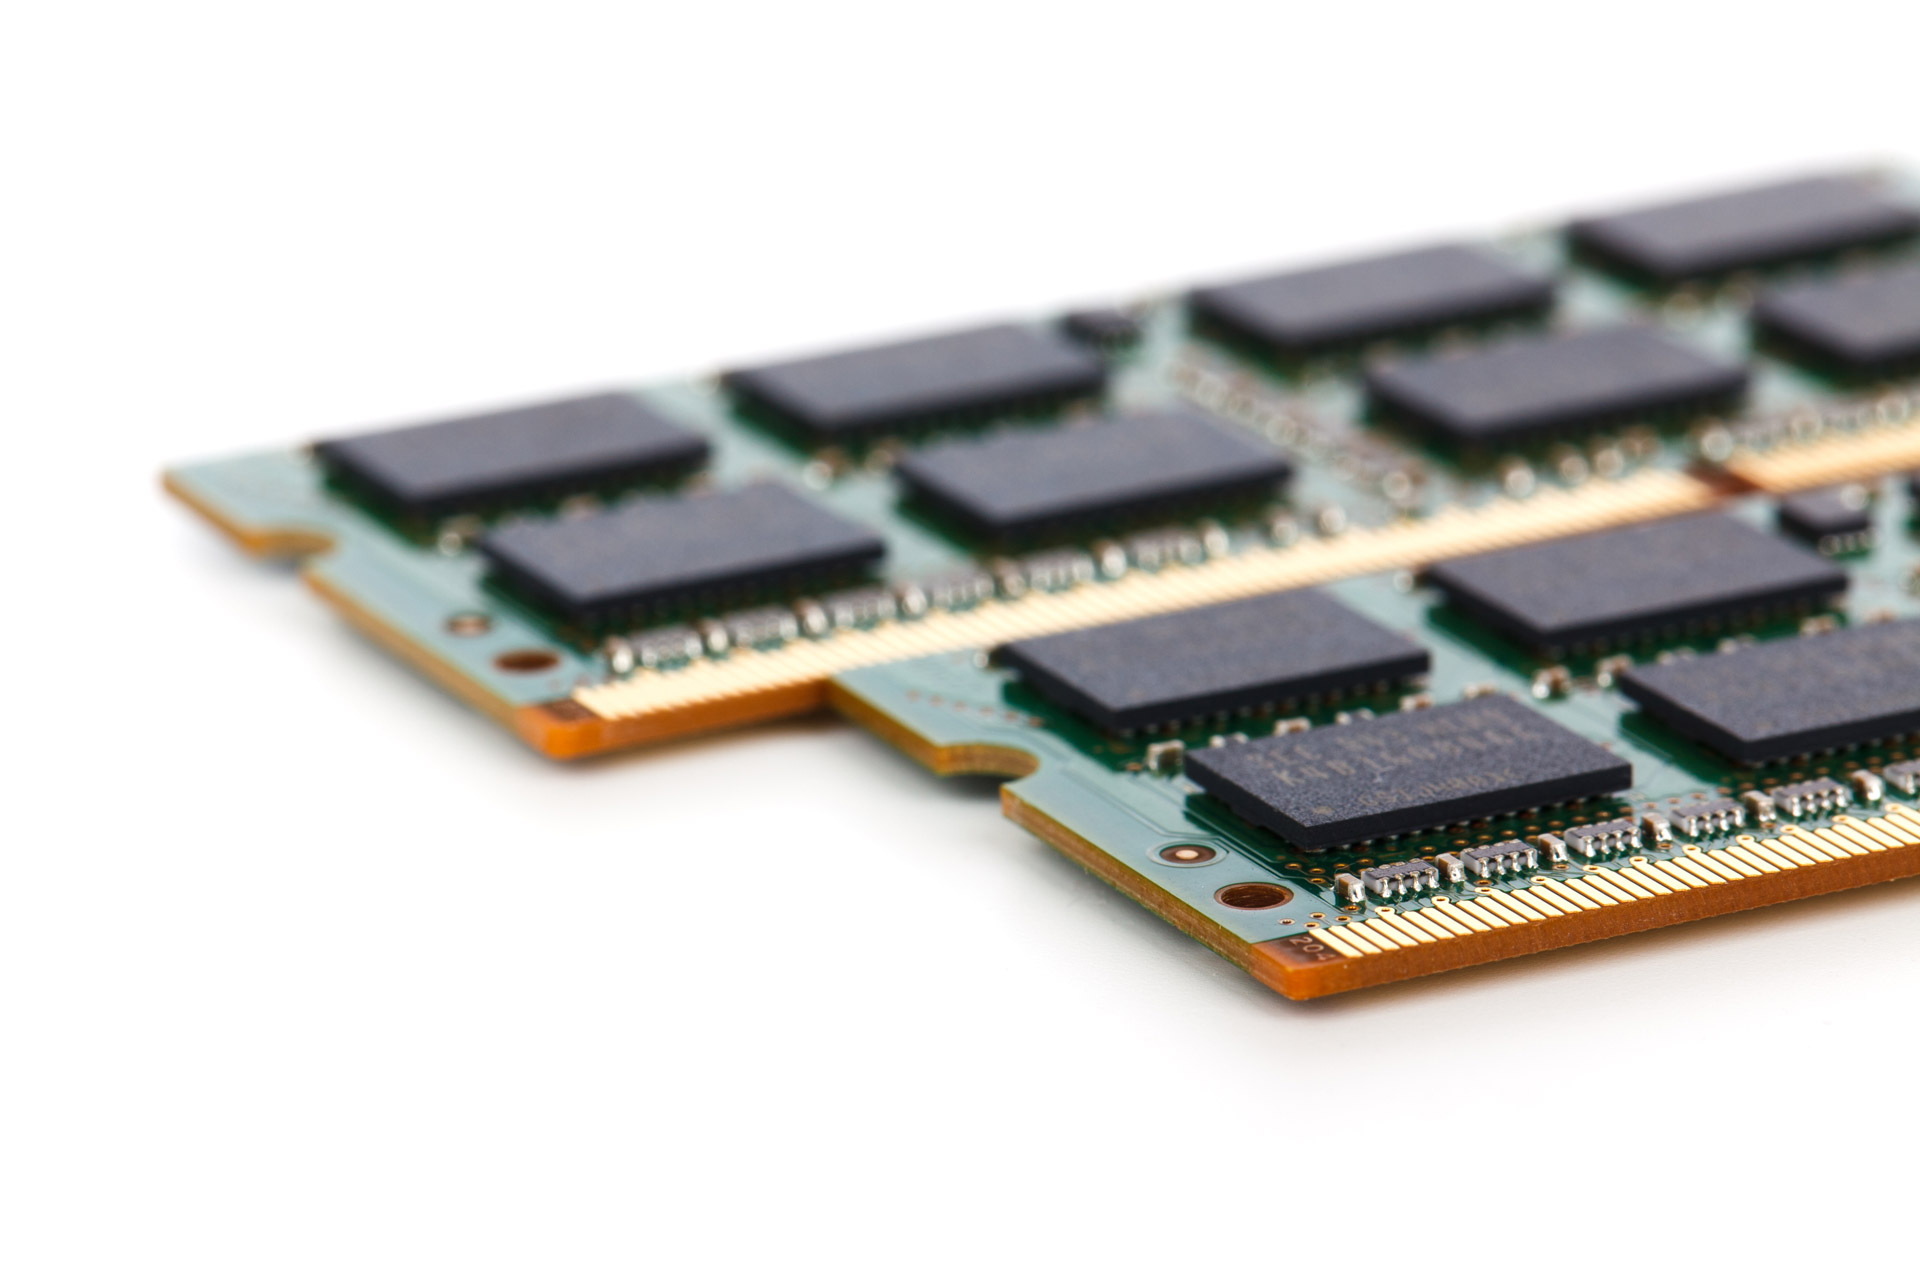
\includegraphics[width=0.70\textwidth]{images/ram.jpg}\\
	\hspace*{15pt}\hbox{\scriptsize Image By:\thinspace{\itshape Petr Kratochvil}}
	%https://www.publicdomainpictures.net/en/view-image.php?image=18285&picture=ram-modules
\end{center}
\end{frame}


% \begin{frame}
	% \frametitle{Function calls}
	% \framesubtitle{Based on a slide by Robbert Krebbers}
	% \begin{columns}
		% \column{0.455\textwidth}
		% \small
		% \textbf{When a function is called:}
		% \begin{itemize}
			% \item A \emph{stack frame} is \emph{added} to memory.
			% \item The stack frame contains:
				% \begin{itemize}
					% \item The function arguments
					% \item The local variables
					% \item The \emph{return address} to track the statement that called the function
				% \end{itemize}
		% \end{itemize}

		% \medskip
		% \textbf{When a function returns:}
		% \begin{itemize}
			% \item The \emph{stack frame} is \emph{removed}.
			% \item Control returns to the \emph{return address}.
		% \end{itemize}
		% \column{0.455\textwidth}

		% \begin{tikzpicture}[
			% node distance=0.2em,
			% stackframe/.style={draw=black,
			% text width=4.5em,minimum height=3em,text centered,font=\small},
			% ]
			% \node[stackframe,fill=green!10] (main) {
				% stack frame for \lstinline|main|
			% };
			% \node[stackframe,above=of main,fill=green!20] (f) {
				% stack frame for \lstinline|f|
			% };
			% \node[stackframe,above=of f,fill=green!30] (g) {
				% stack frame for \lstinline|g|
			% };

			% \node[stackframe,left=0.5em of g,yshift=5em,fill=green!40] (push) {stack frame for \lstinline|h|};
			% \node[stackframe,right=0.5em of g,yshift=5em,fill=green!30] (pop) {stack frame for \lstinline|g|};

			% \draw[->,thick] (push) edge[out=0,in=90] node[left,yshift=-1.5em] {add} ($(g.north)+(-1em,0)$);
			% \draw[<-,thick] (pop) edge[out=180,in=90] node[right,yshift=-1.5em] {remove} ($(g.north)+(1em,0)$);

		% \end{tikzpicture}
	% \end{columns}

	% \pause
	% \begin{columns}[t]
		% \column{0.755\textwidth}

		% \begin{block}{The same function?}
			% Can there be multiple frames for the same function on the stack?
		% \end{block}
		% \pause
		% \column{0.255\textwidth}
		% \begin{block}{Yes!}
			% Recursion!
		% \end{block}
	% \end{columns}
% \end{frame}

\begin{frame}[fragile]{The call stack in action}
	\framesubtitle{Based on a slide by Robbert Krebbers}
\begin{minipage}[t]{0.5\textwidth}
\textbf{Let us call \lstinline|foo(3)|}:

\medskip
\begin{lstlisting}
% [linebackgroundcolor={%
  % \btLstHL<1>{}%
  % \btLstHL<2>{5-8}%
  % \btLstHL<3>{6-8}%
  % \btLstHL<5>{7-8}%
  % \btLstHL<7>{8-8}%
  % \btLstHL<4,6>{2}%
% }]
def bar(n: int) -> int:
  return n;

def foo(n: int) -> int:
	res = 8
	res += bar(n-1) 
	res += bar(n-2) 
	return res
\end{lstlisting}

\medskip
\onslide<2->{
\textbf{When a function is called:}
\begin{itemize}
\item A \emph{stack frame} is \emph{added} to the stack
\item Containing the function arguments, local variables, and the \emph{return address}
\end{itemize}}
\end{minipage}
\hfill
\begin{minipage}[t]{0.48\textwidth}
\textbf{Stack:}

\smallskip
% \begin{tikzpicture}[
  % node distance=0.2em,
  % stackframe/.style={font=\small,draw=structure,thick,fill=structure!0.1,text width=8em},
	% every label/.style={right,font=\scriptsize\tt},
% ]
% \onslide<2->{\node[stackframe,label=right:foo(3),onslide=<2-3>{draw=alert},onslide=<5>{draw=alert},onslide=<7>{draw=alert}] (foo) {
  % \texttt{n} = 3 \\
  % \texttt{res} = \only<2-4>{8}\only<5-6>{10}\only<7->{11} \\
  % \texttt{return}=\emph{main}
% };}

% \onslide<4>{\node[stackframe,label=right:bar(2),above=of foo,onslide=<4>{draw=alert}] (fac2) {
  % \texttt{n} = 2 \\
  % \texttt{return}=line~6
% };}

% \onslide<6>{\node[stackframe,label=right:bar(1),above=of foo,onslide=<6>{draw=alert}] (fac1b) {
  % \texttt{n} = 1 \\
  % \texttt{return}=line~7
% };}

% \invisible{\node[stackframe,label=right:factorial(2),above=of fac1b,onslide=<6>{draw=alert}] (fac2b) {
  % \texttt{n} = 1 \\
  % \texttt{n} = 1 \\
  % \texttt{n} = 1 \\
  % \texttt{return}=line~7
% };}
% \end{tikzpicture}

\medskip
\onslide<4->{
\textbf{When a function returns:}
\begin{itemize}
\item The \emph{stack frame} is \emph{removed}
\item Control returns to the \emph{return address}
\end{itemize}}
\end{minipage}
\end{frame}

\begin{frame}
	\frametitle{A long story short}
	
	Observations:
	\begin{itemize}
		\item Calling a function takes space!
		\item This is important when dealing with recursive functions (which we will discuss after the break).
		\item All of the parameters are stored in this bit of space as well.
	\end{itemize}
	\pause
	\begin{block}{What about lists?}
		Does this mean that the ``stack frame'' for \texttt{baz(my\_list)} requires $O(n)$ space?
	\end{block}
	\pause
	\begin{block}{Nope}
		No! We pass a \textit{reference} instead of a copy. We tell \texttt{baz} where the list is so that it can
		access (or change!) it. Thus this call still requires only $O(1)$ space.\\

		{\scriptsize
		See this excellent StackOverflow post explaining this in more detail if you are interested:
	\url{https://stackoverflow.com/a/986145}.}
	\end{block}
\end{frame}

\begin{frame}
	\frametitle{A second example}
	\framesubtitle{Using a list}
	
	\begin{columns}
		\column{0.455\textwidth}
		\lstinputlisting{src/big-oh-example.py}
		\column{0.455\textwidth}
		\pause
		\begin{block}{Space}
			What is the space complexity of the function \texttt{maya}?
			\begin{enumerate}[A.]
				\item $\Theta(1)$
				\item $\Theta(n)$ 
				\item $\Theta(n^2)$
				\item I don't know.
			\end{enumerate}
		\end{block}
	\end{columns}
	\pause
	\begin{block}{Quadratic space}
		We create a list of $n^2$ items, so we need $\Theta(n^2)$ space. We could say $S(n) = c_0 + c_1n^2$, where $c_0$ is
		for the stack frame, \texttt{s}, \texttt{i} and \texttt{j}. $c_1$ is for \texttt{x}.
	\end{block}
\end{frame}

\begin{frame}
	\frametitle{A second example - modified}
	\framesubtitle{Doing without the list}
	
	\begin{columns}
		\column{0.455\textwidth}
		\lstinputlisting{src/big-oh-example-v2.py}
		\column{0.455\textwidth}
		\pause
		\begin{block}{Space}
			What is the space complexity of the function \texttt{mia}?
			\begin{enumerate}[A.]
				\item $\Theta(1)$
				\item $\Theta(n)$ 
				\item $\Theta(n^2)$
				\item I don't know.
			\end{enumerate}
		\end{block}
	\end{columns}
	\pause
	\begin{block}{Constant space}
		We now only require to store the variable \texttt{s} and call the function \texttt{range}. Both of these require
		constant space, so $S(n) = c_0$ is $\Theta(1)$.
	\end{block}
\end{frame}

\begin{frame}
	\frametitle{A final example - modified}
	\framesubtitle{Using a list from a parameter}
	
	\begin{columns}
		\column{0.455\textwidth}
		\lstinputlisting{src/big-oh-example-v3.py}
		\column{0.455\textwidth}
		\pause
		\begin{block}{Space}
			What is the space complexity of the function \texttt{sum}?
			\begin{enumerate}[A.]
				\item $\Theta(1)$
				\item $\Theta(n)$ 
				\item $\Theta(n^2)$
				\item I don't know.
			\end{enumerate}
		\end{block}
	\end{columns}
	\pause
	\begin{block}{Constant space}
		Remember that a list that is passed as input, is a \textit{reference} and does not take space!
	\end{block}
	\pause
		\begin{block}{Observation}
			Had input contributed to the space complexity, there would be no sub-linear space complexities!	
		\end{block}	
\end{frame}

\begin{frame}
	\frametitle{Relations between time and space?}
	\begin{block}{It's all (a) relative (dimension)}
		Given that a function \texttt{foo} uses $\Theta(n)$ space, what, if anything, can we conclude about the amount of
		time $T(n)$ \texttt{foo} requires?
		\begin{enumerate}[A.]
			\item $T(n)$ is $\Omega(n)$
			\item $T(n)$ is $\Theta(n)$
			\item $T(n)$ is $O(n)$
			\item We cannot conclude anything.
			\item I don't know
		\end{enumerate}
	\end{block}
		\pause
		\begin{block}{A nice lower bound}
			Claiming all of this memory (space) requires time! So we need $\Omega(n)$ time to execute \texttt{foo}!
		\end{block}
\end{frame}

\begin{frame}
	\frametitle{Do your remember?}
	\begin{definition}[Big-Oh]
		A function $f(n)$ is $O(g(n))$ iff there is a positive real constant $c$ and a positive integer $n_0$ such that for
		all $n \geq n_0$ it holds that $f(n) \leq c g(n)$. In other words:\\
		$\exists c \in \mathbb{R}, \exists n_0 \in \mathbb{N} (c > 0 \wedge n_0 \geq 1 \wedge (\forall n \in \mathbb{N} (n
		\geq n_0 \to f(n) \leq cg(n))))$.
	\end{definition}
	\pause
	\begin{columns}
		\column{0.455\textwidth}
		\lstinputlisting{src/big-oh-example.py}
		\pause	
		\column{0.455\textwidth}
		\alt<4>{
			\begin{block}{Run time}
				The run time is described as $T(n) = c_0 + c_1n + c_2n^2$, where
				\begin{itemize}
					\item $c_0$ is for lines 2, 5, and 9.
					\item $c_1n$ is for the range in line 3.
					\item $c_2n^2$ is for lines 4, 5, and 8.
				\end{itemize}
				Thus $T(n)$ is $O(n^2)$.
			\end{block}
			}{
			\begin{block}{So\dots}
				What is a tight upper bound on the run time of \texttt{maya}?
				\begin{enumerate}[A.]
					\item $O(1)$
					\item $O(n)$
					\item $O(n^2)$
					\item $O(n^3)$
					\item I don't know.
				\end{enumerate}
			\end{block}
		}
	\end{columns}
\end{frame}

\begin{frame}
	\frametitle{Which case?}
	\lstinputlisting{src/for-loop-wc.py}
	\begin{columns}
		\column{0.755\textwidth}
	\begin{block}{So which is it?}
		Which of these forms a tight bound on the run time $T(n)$?
	\begin{enumerate}[A.]
		\small
		\item $O(1)$. 
		\item $O(n)$. 
		\item $O(n^2)$. 
		\item I don't know.
	\end{enumerate}	
	\end{block}
		\column{0.255\textwidth}
		\pause
		\begin{block}{}
			Only B
		\end{block}
		\pause
			\begin{block}{Worst Kaas}
				We talk about the \textit{worst-case}.
			\end{block}	
	\end{columns}
\end{frame}

\begin{frame}
	\frametitle{More practice?}
	\begin{itemize}
		\item We will practice this more in tomorrow's tutorial!
		\item As well as big-Oh proofs (i.e. finding $c$ and $n_0$, such that\dots).
	\end{itemize}
\end{frame}

\begin{frame}
	\frametitle{Some python built-in functions}
	\begin{itemize}
		\item You already know about a number of built-in python functions.
			\begin{itemize}
				\item \texttt{range}
			\pause
				\item \texttt{in} (like: \texttt{if $8$ in $x$:})
			\pause
				\item list-comprehensions
			\end{itemize}
			\pause
		\item What is their time complexity?
	\end{itemize}	
\end{frame}

\begin{frame}
	\frametitle{On the topic of ranges}
	\framesubtitle{Get your cowboy boots ready!}

	\begin{columns}
		\column{0.455\textwidth}
			\lstinputlisting{src/range-complexity.py}
		\column{0.455\textwidth}
		\pause
		\begin{block}{GROUP BY}
			Group the different lines by their run time complexity (are they $O(1)$, $O(n)$, $O(n^2)$, etc?)
		\end{block}
	\end{columns}
	\pause
	\begin{block}{So what are they?}
		\begin{enumerate}
			\item $O(n)$, we go through $n$ items.
			\item $O(1)$, there are a constant number of items (100).
			\item $O(n)$, although we go through only $n/2$ items, this still grows linearly as $n$ grows.
			\item $O(1)$, this is again a constant number of items (100).
		\end{enumerate}
	\end{block}
\end{frame}

\begin{frame}
	\frametitle{What about in?}
	\framesubtitle{Everyone get in here!}

	\begin{columns}
		\column{0.455\textwidth}
			\lstinputlisting{src/in-complexity.py}
		\column{0.455\textwidth}
		\pause
		\begin{block}{Searching}
			What is the time complexity of this operation?
			\begin{enumerate}[A.]
				\item $O(1)$
				\item $O(n)$ where $n = $\texttt{len(my\_list)}.
				\item $O(n^2)$ where $n = $\texttt{len(my\_list)}.
				\item I don't know.
			\end{enumerate}
		\end{block}
	\end{columns}
	\pause
	\begin{block}{Linear time}
		Worst case we need to check every element, so $O(n)$ time.
	\end{block}
\end{frame}

\begin{frame}
	\frametitle{List comprehensions}
	\framesubtitle{Comprehende?}

	\begin{columns}
		\column{0.455\textwidth}
			\lstinputlisting{src/comprehension-complexity.py}
		\column{0.455\textwidth}
		\pause
		\begin{block}{Comprehension}
			What is the time complexity of this list comprehension?
			\begin{enumerate}[A.]
				\item $O(1)$
				\item $O(n)$ 
				\item $O(n^2)$
				\item I don't know.
			\end{enumerate}
		\end{block}
	\end{columns}
	\pause
	\begin{block}{Linear time}
		The answer is in the for loop. This is $O(n)$ and so the creation of the list is also $O(n)$. 
	\end{block}
	\pause
		\begin{block}{Why though?}
			We will see why exactly when we discuss lists next week.
		\end{block}	
\end{frame}

\begin{frame}
	\frametitle{More bounds}
	\begin{center}
		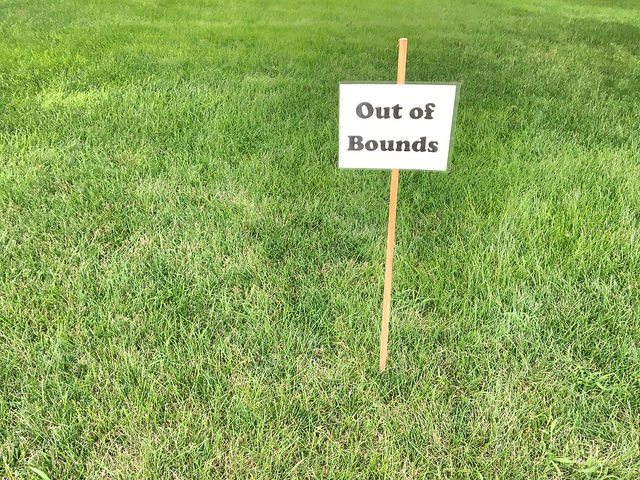
\includegraphics[width=0.6\textwidth]{images/bounds.jpg}\\
		\hspace*{15pt}\hbox{\scriptsize Image By:\thinspace{\itshape David Mulder}}
		%https://www.flickr.com/photos/113026679@N03/43459273171
	\end{center}
\end{frame}

\begin{frame}
	\frametitle{A lower bound}
	\framesubtitle{Omega}
	\begin{definition}[Big-$\Omega$ (Omega)]
		A function $f(n)$ is $\Omega(g(n))$ iff there is a positive real constant $c$ and a positive integer $n_0$ such that for
		all $n \geq n_0$ it holds that $f(n) \geq c g(n)$. In other words:\\
		$\exists c \in \mathbb{R}, \exists n_0 \in \mathbb{N} (c > 0 \wedge n_0 \geq 1 \wedge (\forall n \in \mathbb{N} (n
		\geq n_0 \to f(n) \geq cg(n))))$.
	\end{definition}
	\pause
	\begin{block}{What of it?}
		Assume that $f(n)$ is $O(g(n))$ what, if anything, can we now conclude?
		\begin{enumerate}[A.]
			\item $f(n)$ is $\Omega(g(n))$
			\item $g(n)$ is $O(f(n))$
			\item $g(n)$ is $\Omega(f(n))$
			\item None of the above.
			\item I don't know.
		\end{enumerate}
	\end{block}
\end{frame}

\begin{frame}
	\frametitle{So what?}
	\begin{block}{Why do we care?}
		What can we use big-$\Omega$ for?
	\end{block}
	\pause
	\begin{block}{Not much!}
		Very very little :) \\
		\pause
		Though occassionally we can prove things require e.g.\ $\Omega(n)$ steps, even if we do not know how to solve it
		exactly.\\
		\pause
		But if something is both $O(f(n))$ and $\Omega(f(n))$\dots
	\end{block}
	\pause
	\begin{definition}[Big-$\Theta$ (Theta)]
		A function $f(n)$ is $\Theta(g(n))$ iff there are positive real constants $c_0, c_1$ and a positive integer $n_0$ such that for
		all $n \geq n_0$ it holds that $c_0 g(n) \leq f(n) \leq c_1 g(n)$. In other words:\\
		{\small
		$\exists c_0,c_1 \in \mathbb{R}, \exists n_0 \in \mathbb{N} (c_0> 0 \wedge c_1 > 0\wedge n_0 \geq 1 \wedge (\forall
		n \in \mathbb{N} (n \geq n_0 \to c_1 g(n) \leq f(n) \leq c_2 g(n))))$.
	}
	\end{definition}
\end{frame}

\begin{frame}
	\vspace{-10pt}
	\begin{overlayarea}{\textwidth}{\textheight}
			\begin{block}{Why do we care about this?}
				So is big-$\Theta$ any use?
			\end{block}
			\pause
	\vspace{-5pt}
			\begin{block}{Yes!}
				It is basically the ``tight upper bound'' we discussed yesterday.
			\end{block}
			\pause
	\vspace{-5pt}
		\only<-5>{
			\begin{columns}
				\column{0.455\textwidth}
				\lstinputlisting{src/big-oh-example.py}
				\pause	
				\column{0.455\textwidth}
				\alt<5>{
					\begin{block}{Run time}
						The run time is described as $T(n) = c_0 + c_1n + c_2n^2$, where
						\begin{itemize}
							\item $c_0$ is for lines 2, 5, and 9.
							\item $c_1n$ is for the range in line 3.
							\item $c_2n^2$ is for lines 4, 5, and 8.
						\end{itemize}
						Thus $T(n)$ is $\Theta(n^2)$.
					\end{block}
					}{
					\begin{block}{So\dots}
						What is a tight bound on the run time of \texttt{maya}?
						\begin{enumerate}[A.]
						\small
							\item $\Theta(1)$
							\item $\Theta(n)$
							\item $\Theta(n^2)$
							\item $\Theta(n^3)$
							\item I don't know.
						\end{enumerate}
					\end{block}
				}
			\end{columns}
		}
		\only<6>{
				\begin{alertblock}{Despite all that...}
					We still often \textit{just} ask for ``a tight upper bound'' and will accept a big-Oh.
				\end{alertblock}	
		}
	\end{overlayarea}
\end{frame}
